% Chapter Template

\chapter{Organizations and Components} % Main chapter title

\label{Chapter3} % Change X to a consecutive number; for referencing this chapter elsewhere, use \ref{ChapterX}

\lhead{Chapter 3. \emph{Organizations and Components}} % Change X to a consecutive number; this is for the header on each page - perhaps a shortened title

This chapter enumerates the components constituting the PubSeq system and explains how each in principle functions. There would also be technicalities of the programs and rationales on how each of the component is used and implemented.

%----------------------------------------------------------------------------------------
%	SECTION 1
%----------------------------------------------------------------------------------------

\section{Introduction}

\label{sec:Chap3Intro}

In the most general term, there are three main components that build up the PubSeq environment. The three components could be represented as questions:

\begin{itemize}
\item How to \textit{create} the data?
\item How the data is going to be \textit{stored}?
\item How the user is going to \textit{retreive} the data?
\end{itemize}

We \textit{create} the data in which we process the raw data from our source into indexable entry data. We then \textit{store} the data in scalable manner for the user to use. Finally, we will facilitate how a user could \textit{retreive} our data.

We formalize this concept further by creating three main components with each represents the answer of the question before:

\begin{itemize}
\item \textbf{PubSeq Tagging Pipeline} (\textbf{Tagging Pipeline} for short) addresses the first question. In this pipeline we would process the data from its main source, the MEDLINE corpus which is updated daily as XML file, onto indexable input file containing list of UniProt annotations in the abstracts, among others.
\item \textbf{PubSeq Solr Index} (\textbf{Solr Index} for short) addresses storage issue. All processed data would then in an open source enterprise search platform, Solr \citep{smiley2015apache}.
\item \textbf{PubSeq Web Server} (\textbf{Solr Server}) addresses the issue of content delivery to end user. Here we would explain the program in more technical manner. We would also convey how the program would see in the perspective of end user -- that is how the program runs as user proceeds on using the search engine, later in Chapter \ref{Chapter6}.
\end{itemize}

%----------------------------------------------------------------------------------------
%	SECTION 2
%----------------------------------------------------------------------------------------

\section{PubSeq Persistent Components}

To understand how the components were structured, I think it is better for the reader to first get to know how the persistent components, that is, the components that are running around-the-clock interact:

\begin{figure}[htbp]
  \centering
    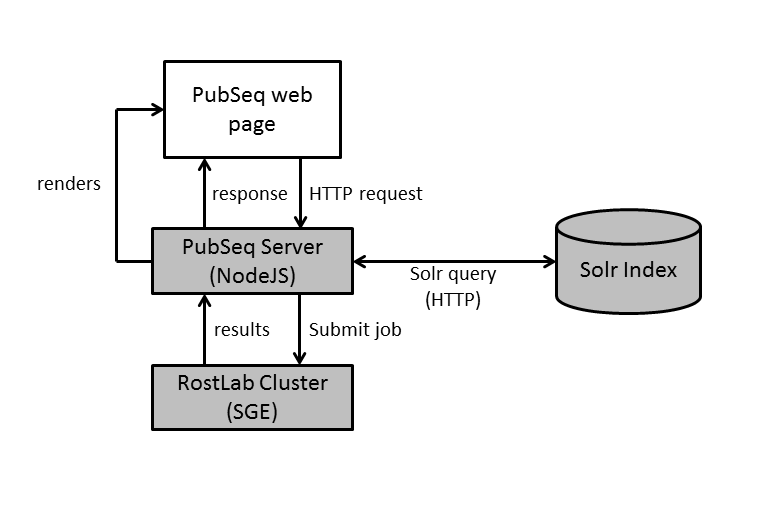
\includegraphics[width=6in]{Figures/solr_graph_main.png}
    \rule{35em}{0.5pt}
  \caption[An Overview of how the 'Persistent Components' of PubSeq environment interacts.]{An overview of how the Persistent Components -- the components that are running around the clock -- interact with each other. Here we can see two of three main components explained before: Solr Index, Solr Server (and its rendered web app instance, PubSeq Web Page) which is also connected with RostLab Cluster via SunGrid Engine (SGE). Compare this diagram with spatially differentiated diagram of the system with Virtual Machine shown (Figure \ref{fig:PubSeqVM} in Chapter 6)}
  \label{fig:ComponentInteraction}
\end{figure}

Here we can see three main components within the interaction environment: Solr Index, PubSeq Server, PubSeq web page and RostLab Cluster (SunGrid Engine).

\begin{itemize}
\item \textbf{PubSeq Web Page} is rendered by PubSeq server upon GET request on PubSeq home path and communicates through HTTP protocols to PubSeq server. There are currently POST and GET methods that are launched by this page onto the server. Beside the server, the PubSeq web server, the web page also presents some links to outside world, most notably to PubMed web interface \citep{MELDINEWeb}. The linkage to PubMed web interface was embeded in each of the results of the query within PubSeq (see Chapter \ref{Chapter6} for details)
\item \textbf{PubSeq Web Server} is server component of our system. It handles HTTP requests addressed to the web path and renders PubSeq web page. Internally it processes both queries and results from both web page and server reply. The server also communicates to RostLab's clusters for submitting BLAST query for a given sequence.
\item \textbf{PubSeq Solr Index} contains the whole indexing of MEDLINE and proteins mentions within article. While the main mechanism of updating the index will be explained thoroughly in later chapter, it is important to know for reader that the index only communicates via HTTP \citep{smiley2015apache}. As thus, user can check on the machine that the server runs on, the sample content of the Solr server by doing curl followed by the query. For more details see dedicated chapters bellow.
\item We utilize \textbf{RostLab Cluster} for BLASTing input sequence given by the user.
\end{itemize}

%----------------------------------------------------------------------------------------
%	SECTION 3
%----------------------------------------------------------------------------------------

\section{Web Interaction}

We model our web interaction in following time-dependent sequence diagram \citep{rumbaugh2004unified} on Figure \ref{fig:SequenceDiagram}.

\begin{figure}[htbp]
  \centering
    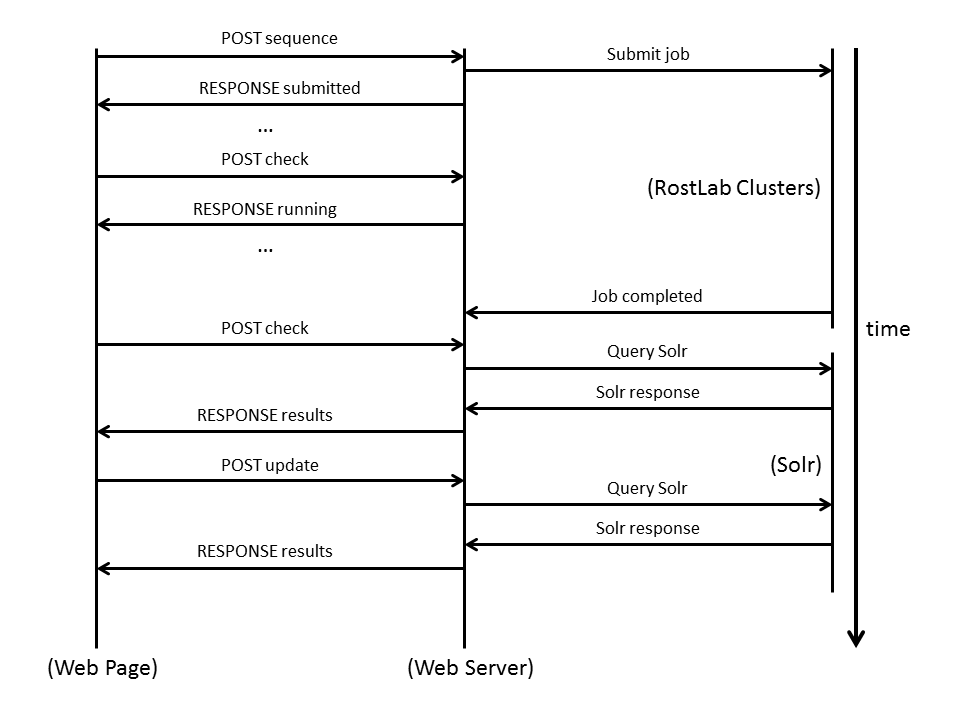
\includegraphics[width=6in]{Figures/sequence_diagram.png}
    \rule{35em}{0.5pt}
  \caption[A Sequence Diagram modeling of PubSeq web interaction.]{Time-dependent sequence diagram of PubSeq web interaction. The y-axis represents the time (from top to bottom) and each of the columns in on the x-axis represents components that interact with each others. Note that the in the third column, there are two entities that interact with Web Server in distinct time spans.}
  \label{fig:SequenceDiagram}
\end{figure}

Here we see how four main persistent components of PubSeq interact. First, the user opens the PubSeq page. This will spawn an instance of PubSeq web page. Upon inserting some sequence and pressing query button, the web page would then submit the initial HTTP request \citep{fielding1999hypertext} onto the server (first \textbf{POST sequence}). Our Node.js server \citep{tilkov2010node} would then handle the query and create a script and input file containing aforementioned sequence. It would then submit the query onto RostLab cluster through qsub (\textbf{Submit job}) \citep{gentzsch2001sun} and return first response containing message informing the web client that the job has been submitted (\textbf{RESPONSE submitted}). The web client would then re-check the server once in a while (ca. 10 seconds) to find out whether the result of the query has been created (\textbf{POST check} and \textbf{RESPONSE running}). Once the job has been completed the results would be saved in a pre-defined location using pre-defined names (see later chapter for more details). During the next iteration of checking routine from web app, if the output is already there, the request handler would then parse the output file and prepare a Solr query that would be used for the sequence. This query would then be submitted onto Solr client (\textbf{Query Solr}). The query response would then be forwarded to web page in the RESPONSE massage (\textbf{RESPONSE results}) and the results would be shown to the user. Had the user have to update the results (mostly by moving between result pages), an update POST would be initiated (\textbf{POST sequence}). This update POST contains prepared statement that doesn't require another BLAST, and thus would be directed toward Solr index directly (second \textbf{Query Solr}). Just like initial Solr response, the resulting query would be returned to user. As long as user doesn't leave the page or query new sequence, this iteration could be done as many times as possible.

%----------------------------------------------------------------------------------------
%	SECTION 4
%----------------------------------------------------------------------------------------

\section{Tagging Pipeline}

Tagging pipeline refers to the process of creating and updating the Solr index that would be used for the server to search for articles containing protein mentions. In this pipeline, a set of documents from MEDLINE database would sequentially processed and finally be pushed into our index. The whole process is done in periodic/one-off basis. The schematic representation with each single step obscured can be seen in Figure \ref{fig:TaggingPipelineBroad}.

\begin{figure}[htbp]
  \centering
    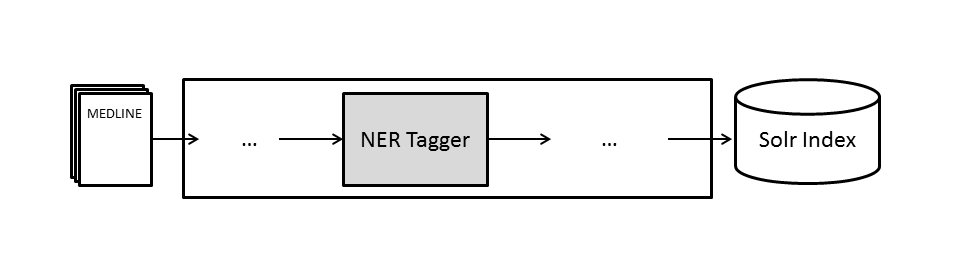
\includegraphics[width=6in]{Figures/solr_tagging_pipeline.png}
    \rule{35em}{0.5pt}
  \caption[Schematic representation of PubSeq Tagging Pipeline.]{Schematic diagram representing the broad process of Solr Tagging Pipeline. On the left side the input files, MEDLINE abstracts in XML formats, would be processed sequentially until the data is ready to be pushed onto the Solr index. We deliberately highlighted NER Tagging from within the pipeline to emphasize its importance in our pipeline.}
  \label{fig:TaggingPipelineBroad}
\end{figure}

Here we see that the process consists of smaller processes. As already said, there could be two way of running this process: one-off and periodic update. While one-off Tagging Pipeline could be done on RostLab's \textbf{jobtest}/\textbf{jobtest2} or similar physical servers within RostLab infrastructure, the periodic update process should be only done via SunGrid Engine call scheduled in crontab \citep{keller1999take}.

We deliberately showed the NER Tagger process within this Pipeline to reader to emphasize its importance. Lars Juhl Jensen was kind enough to give us his program that we use to run on our pipeline. There would be more details on both our NER Tagger and Tagging Pipeline in later chapter(s) but for now we would focus on big picture detail.